\documentclass[12pt]{article}
\usepackage{graphicx, epstopdf}

\begin{document}
\title{Summary report of rejection email analysis}
\author{Davide Chiuchiu}

\maketitle

\section{Scope}
This document contains my findings on the corpus of emails that I received during my job search. The email database contains 
\begin{itemize}
	\item the emails that confirmed the application submission
	\item the emails where companies showed interest in pursuing further my candidacy
	\item the emails where companies rejected my candidacy.
\end{itemize}

\section{I received more confirmation emails than rejection emails}
The first thing that I notice from this dataset is that I received more emails which confirmed the reception of my candidacy than rejection emails (see Figure \ref{fig:email_type_distribution}). This highlight that I have active review process at the moment, but also that some companies practice ghosting. Note also that only a few of the received emails corresponds to feedback. This means that I will likely need to ignore feedback emails in machine learning approaches for this analysis.

\begin{figure}[tb!]
	\center
	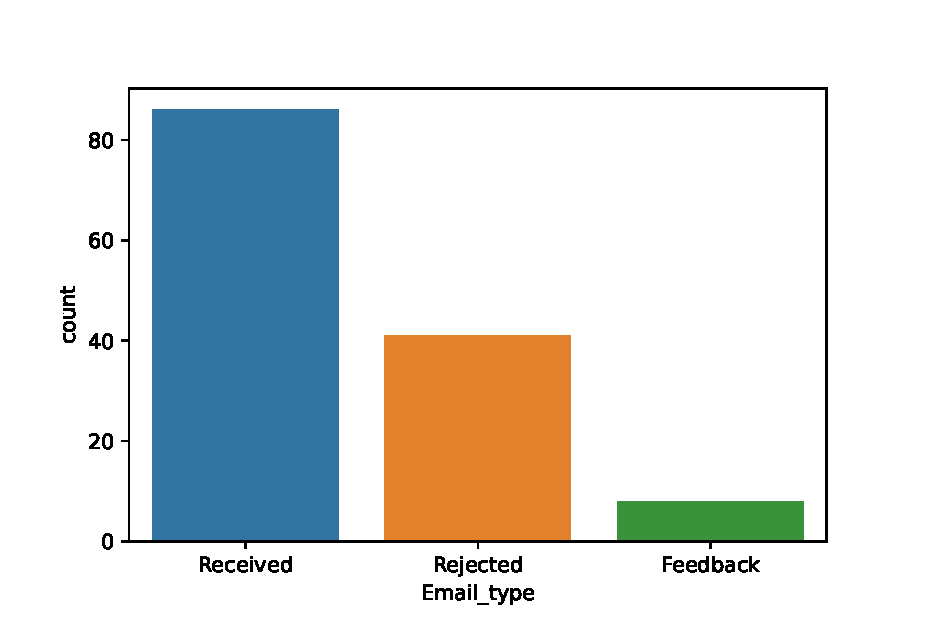
\includegraphics[width = 0.5\linewidth]{email_type_distribution.eps}
	\caption{I received more emails which confirms that my candidacy has been received than  emails where my candidacy was rejected. Unfortunately, only a small subset of emails correspond to feedback from potential employers. \label{fig:email_type_distribution}}
\end{figure}

\section{Candidate feedback might suffer because rejection emails tend to be quite short.}
Candidates may not receive extensive feedback for failed submissions. Indeed, emails where candidacies have been rejected tend to be shorter than feedback emails (see Figure \ref{fig:email_lengths}). In addition, the emails which rejects a candidacy and the template emails that acknowledge a candidacy submission tend to have similar lengths. This feature suggests that emails where candidacies are rejected often corresponds to templates that leaves unsuccessful candidates without constructive feedback. 

\begin{figure}
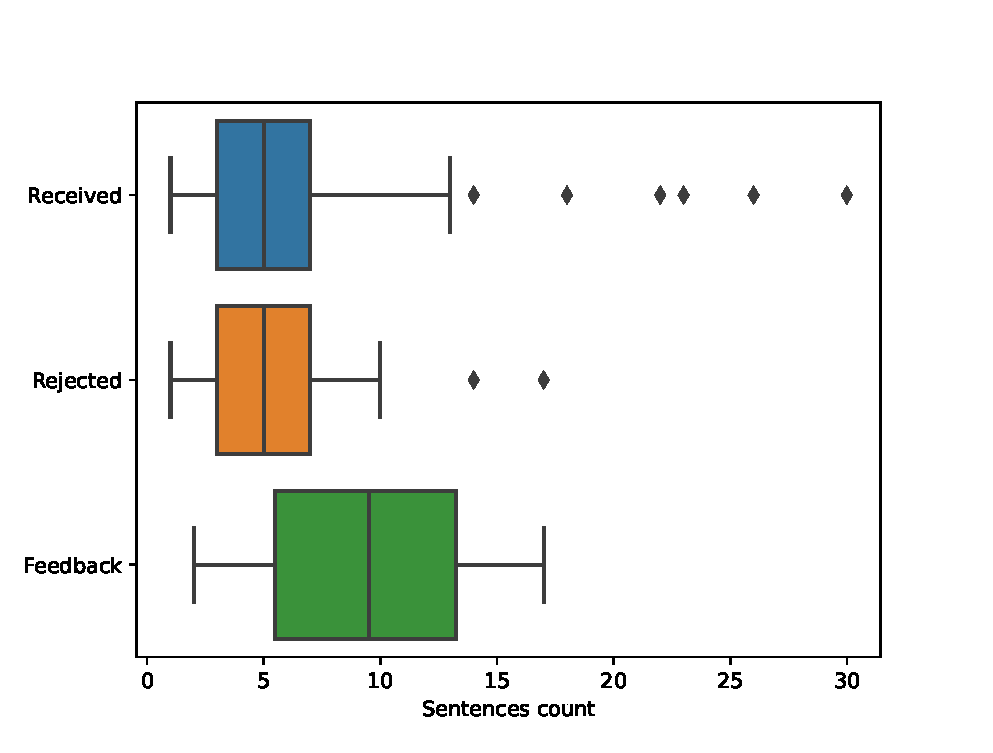
\includegraphics[width = \linewidth]{message_length_distribution.eps}
\caption{Unsuccessfull applicants may recieve little constructive feedback when they are rejected because the rejection emails are quite short. \label{fig:email_lengths}}
\end{figure}

\end{document}